%=========================================================
\chapter{Modelo dinámico}	


El modelo dinámico es una parte fundamental en el diseño de sistemas de software, ya que se centra en capturar y representar el comportamiento y las interacciones del sistema a lo largo del tiempo. Este modelo nos permite comprender cómo los diferentes componentes del sistema interactúan entre sí y cómo se llevan a cabo las acciones y procesos. En el contexto del sistema de la "Guardería burbujas", el modelo dinámico nos ayudará a visualizar y analizar el flujo de eventos y el comportamiento en tiempo real del sistema.

El objetivo principal del modelo dinámico en el sistema de la "Guardería burbujas" es describir las secuencias de acciones y eventos que ocurren durante la ejecución del sistema. Esto implica identificar las interacciones entre los diferentes actores, como los usuarios y el sistema, y cómo se desarrollan las acciones a lo largo del tiempo. El modelo dinámico nos permite comprender cómo se realizan las transiciones entre los diferentes estados del sistema y cómo se gestionan los flujos de información y control.
\\

Al diseñar el modelo dinámico del sistema de la "Guardería burbujas", se utilizan diferentes técnicas y diagramas para representar las secuencias de acciones y eventos. Uno de los diagramas más utilizados es el diagrama de secuencia, que muestra la interacción entre los diferentes objetos del sistema en función del tiempo. Este diagrama permite visualizar el orden y la duración de las acciones, así como las relaciones entre los objetos involucrados.

El modelo dinámico en el sistema es esencial para comprender y visualizar el comportamiento del sistema en tiempo real. Permite identificar los flujos de acciones y eventos, así como los procesos que se llevan a cabo durante la ejecución del sistema. Un diseño adecuado del modelo dinámico garantiza un sistema eficiente, confiable y orientado a las necesidades de los usuarios.

\newpage
\section{Diagrama de secuencia del CU1:Registrar profesor}


\begin{figure}[htbp]
\centering
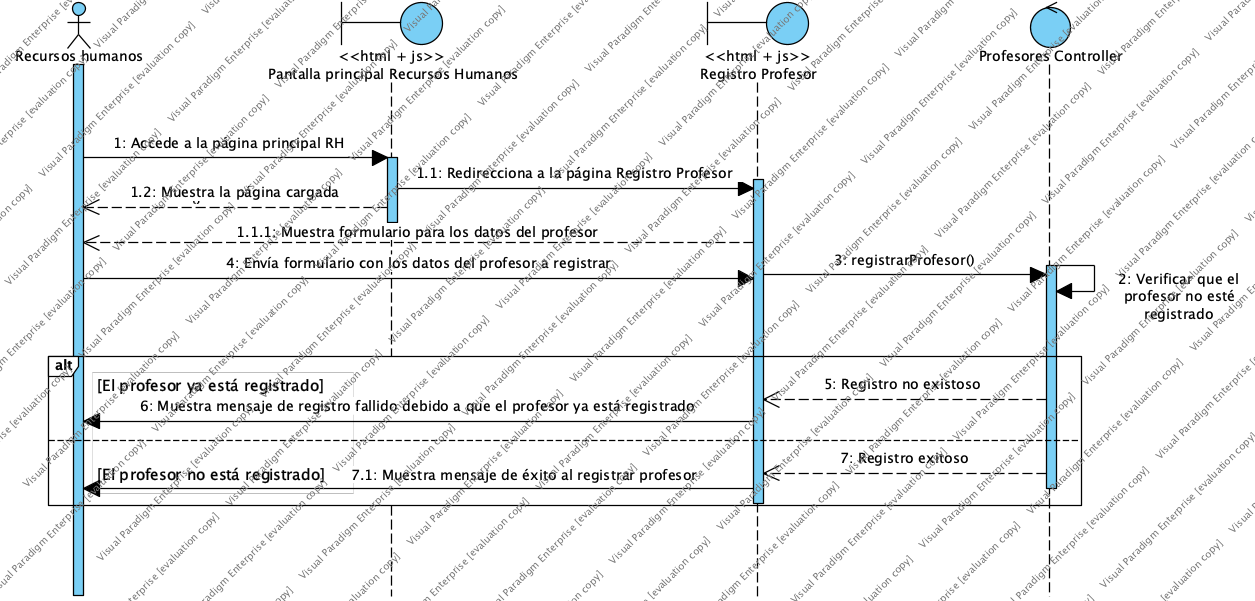
\includegraphics[width=0.7\textwidth]{images/diagramaSecuenciaCU1.png}
\caption{Diagrama de secuencia del CU1.}
\label{fig:diagramaSecuenciaCU1}
\end{figure}

\section{Diagrama de secuencia del CU4:Enlazar niño con padre}


\begin{figure}[htbp]
\centering
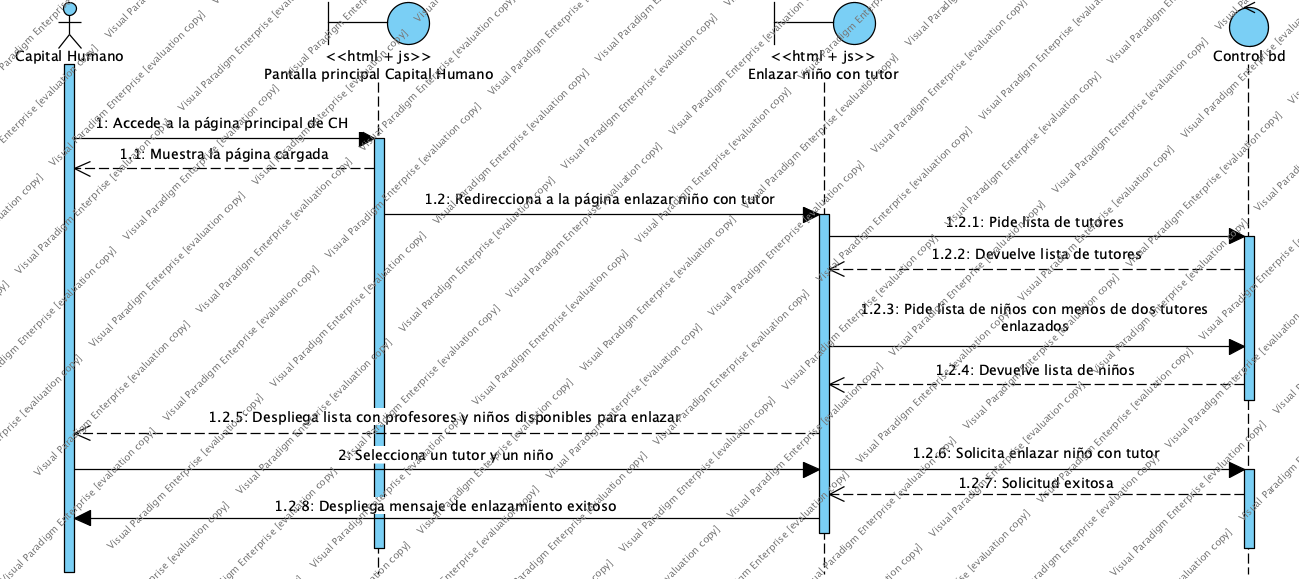
\includegraphics[width=0.7\textwidth]{images/diagramaSecuenciaCU4.png}
\caption{Diagrama de secuencia del CU4.}
\label{fig:diagramaSecuenciaCU4}
\end{figure}

\newpage
\section{Diagrama de secuencia del CU5:Registrar profesor}


\begin{figure}[htbp]
\centering
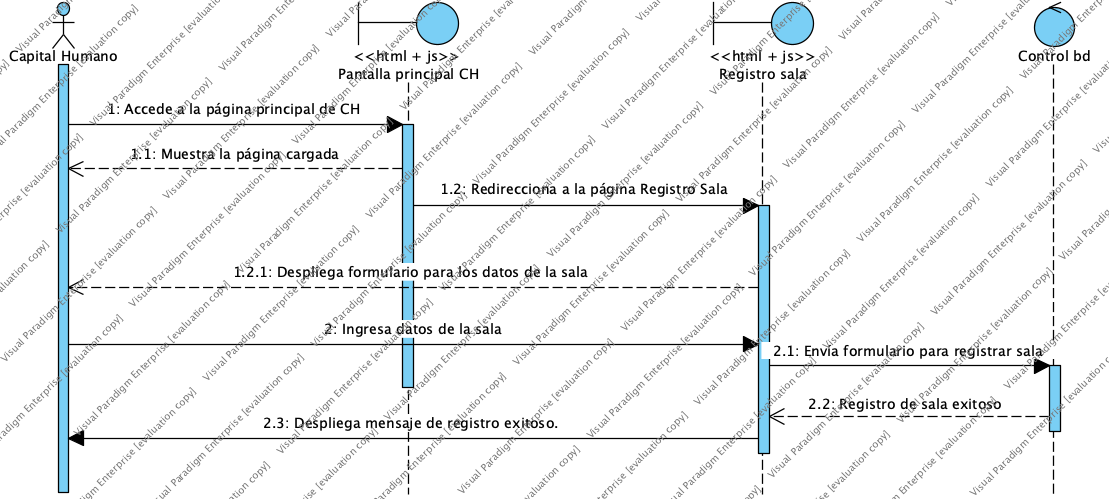
\includegraphics[width=0.7\textwidth]{images/diagramaSecuenciaCU5.png}
\caption{Diagrama de secuencia del CU5.}
\label{fig:diagramaSecuenciaCU5}
\end{figure}

\section{Diagrama de secuencia del CU7:Enlazar niño con padre}


\begin{figure}[htbp]
\centering
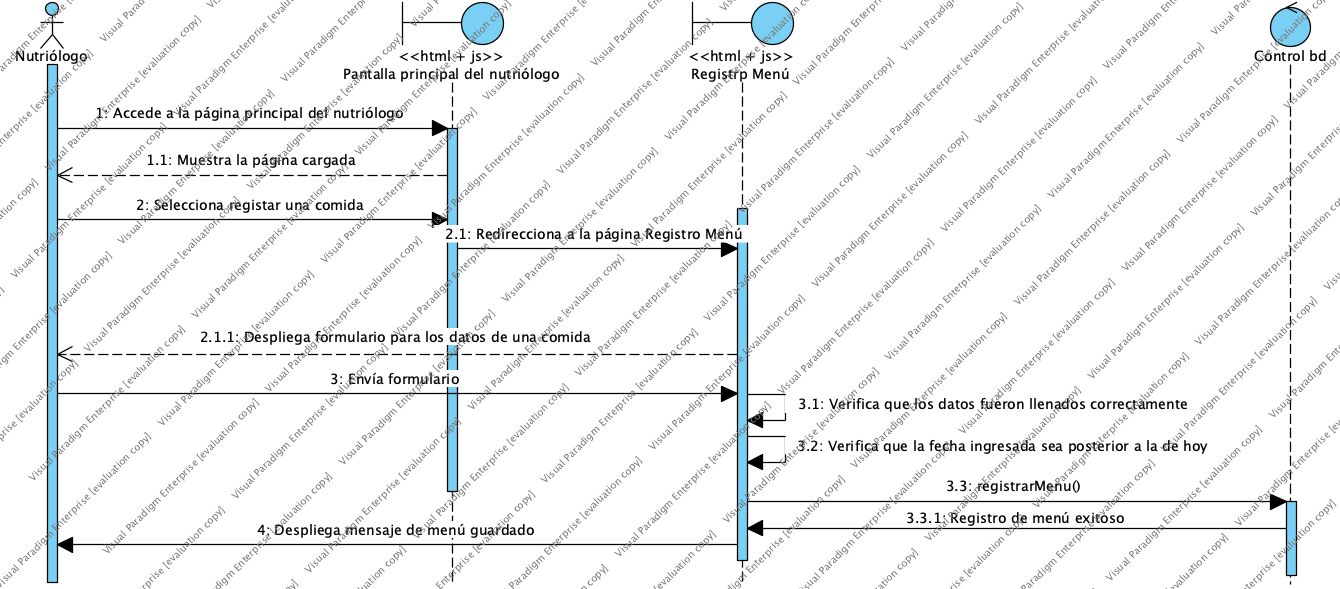
\includegraphics[width=0.7\textwidth]{images/diagramaSecuenciaCU7.png}
\caption{Diagrama de secuencia del CU7.}
\label{fig:diagramaSecuenciaCU7}
\end{figure}

\newpage
\section{Diagrama de secuencia del CU9:Registrar ingesta}

\begin{figure}[htbp]
\centering
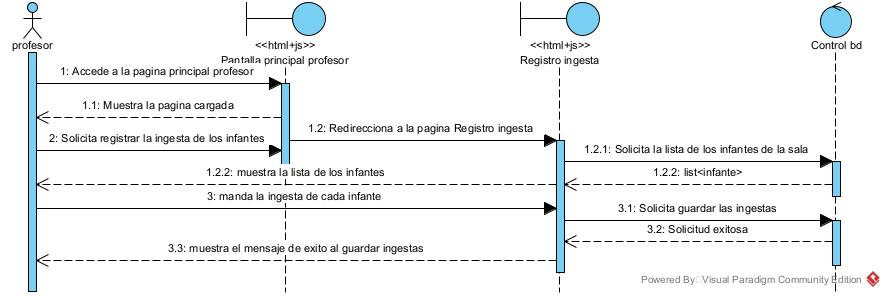
\includegraphics[width=0.7\textwidth]{images/diagramasecuencia9.jpg}
\caption{Diagrama de secuencia del CU9.}
\label{fig:diagramasecuencia9}
\end{figure}

\section{Diagrama de secuencia del CU12:Registrar tarea}

\begin{figure}[htbp]
\centering
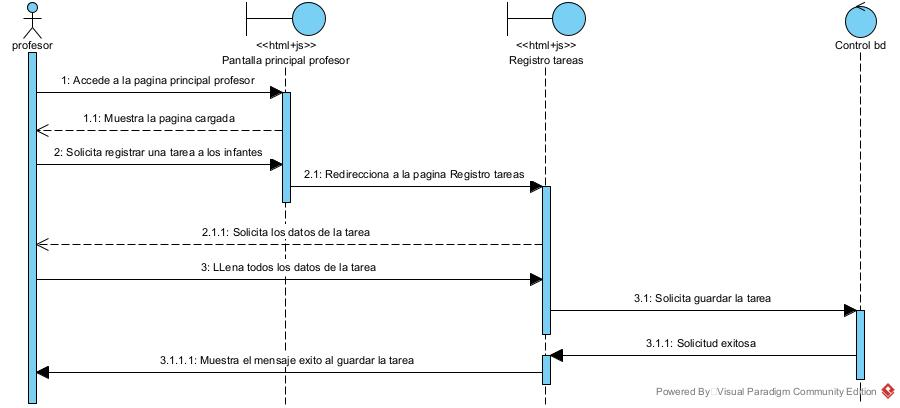
\includegraphics[width=0.7\textwidth]{images/diagramasecuencia12}
\caption{Diagrama de secuencia del CU12.}
\label{fig:diagramasecuencia12}
\end{figure}

\newpage
\section{Diagrama de secuencia del CU15:Registrar incidencia medica}

\begin{figure}[htbp]
\centering
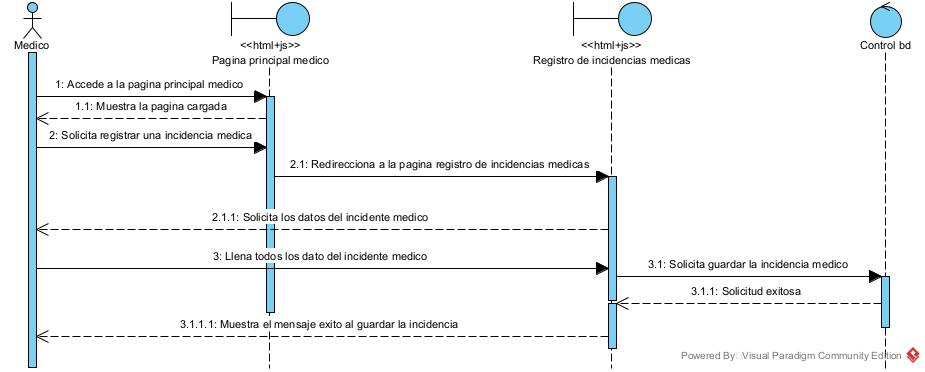
\includegraphics[width=0.7\textwidth]{images/diagramasecuencia15}
\caption{Diagrama de secuencia del CU15.}
\label{fig:diagramasecuencia15}
\end{figure}

\section{Diagrama de secuencia del CU19:Tomar asistencia}

\begin{figure}[htbp]
\centering
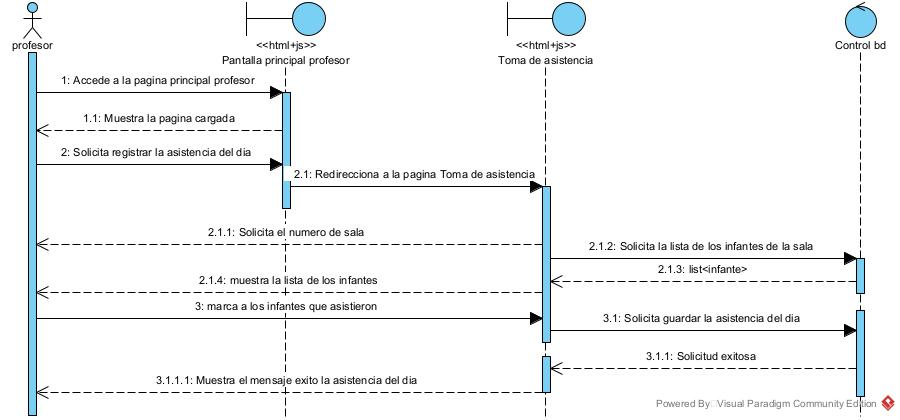
\includegraphics[width=0.7\textwidth]{images/diagramasecuencia19}
\caption{Diagrama de secuencia del CU19.}
\label{fig:diagramasecuencia19}
\end{figure}